\documentclass[10pt, a5paper]{article}
\usepackage{fontspec}
\usepackage{tabularx}
%\usepackage{array}
\usepackage[usenames,dvipsnames]{xcolor}
\usepackage[bookmarks, colorlinks, breaklinks]{hyperref}
\hypersetup{linkcolor=blue,citecolor=blue,filecolor=black,urlcolor=MidnightBlue} 
\begin{document}

\section{Introduction to Molecular Dynamics}

\begin{itemize}
\item
The interaction between molecules is represented by the interaction law specified by the potential $U(r_1,\dots, r_N)$ (aka force field) representing the potential enery of N interacting atoms as a function of their positions in 3D space $r_i = (x_i, y_i, z_i)$ \cite{meller-2001}.

% figure 
\noindent\begin{tabularx}{\textwidth}{X}
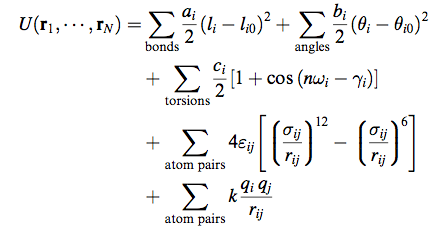
\includegraphics[scale=.5]{figures/ff-eqn1.png} \\
 \tiny{Typical force-field used in biosystem simulations }\\
\end{tabularx}

\item 
Another set of equations used in MD simulate Potential Enenergy 
\begin{equation}
 E_P(x) = E_{bonded} + E_{non-bonded}
 \end{equation}

\item
\emph{ab initio} (from the beginning) Born-Oppenheimer:\\
In quantum chemistry, the computation of the energy and the wavefunction of an average-size molecule is a formidable task that is alleviated by the Born–Oppenheimer (BO) approximation, named after Max Born and J. Robert Oppenheimer[\href{http://en.wikipedia.org/wiki/Born–Oppenheimer_approximation}{from wikipedia}]


\item 
van-der-Waals

\item 
Energy minimazation 

\item 
\href{http://www.physics.sc.edu/~knight/502s08/SE.pdf}{Schrodinger Equation}
\href{http://farside.ph.utexas.edu/teaching/315/Waves/node72.html}{One dimensional wave-function mathematical representation}

	\begin{equation}
	\psi(x,t) = A\,\cos(\phi+k\,x-\omega\,t),
	\end{equation}

\end{itemize}
\section{Molecular Dynamics - Multi-media}

\end{document}
